% ASPLOS 2027 mandates: sigplan + anonymous + review + nonacm.
% 10pt is stated explicitly as well: the CFP requires 10pt body text (not 9pt).
\documentclass[sigplan,review,nonacm,10pt]{acmart}
\settopmatter{printacmref=false}
\acmConference[ASPLOS '27]{ACM International Conference on Architectural Support for Programming Languages and Operating Systems}{April 11--15, 2027}{Heraklion, Crete, Greece}
% (acmart's own Libertine/newtx fonts are used: no lmodern override)
\setlength{\emergencystretch}{2em}
% \Bbbk is already provided when acmart loads newtxmath; let amssymb redefine it
% cleanly instead of erroring on TeX installations that have both.
\let\Bbbk\relax
\usepackage{amssymb}
\usepackage{booktabs}

\begin{document}
\title{The Lock-Step Tax: Per-Lane Control Flow as the Missing Primitive in Tile GPU DSLs}
\author{Alessandro Potenza}
\affiliation{\institution{Politecnico di Milano}\city{Milan}\country{Italy}}
\email{alessandro1.potenza@mail.polimi.it}
\renewcommand{\shortauthors}{Potenza}

\begin{abstract}
Tile abstractions are how GPU kernels are written now, in Triton and increasingly in the
vendor's own stack, and on dense tensor work they match hand-written CUDA. On irregular,
control-driven kernels they lose an order of magnitude. Whether that gap is a tuning
deficit or a property of the abstraction is a question about language design, and it has
not been answered mechanistically.

We answer it. The gap is structural, and one shared loop latch explains it. A tile
program's lanes advance together, so a data-dependent loop runs as long as its warp's
slowest lane and a dependent load cannot be overlapped across lanes. On an NFA worklist
the gap decomposes into a launch-configuration artifact, a redundancy removable by
lane-packing, and an irreducible ${\sim}2\times$ residual. At matched occupancy, issuing
\emph{fewer} warp-instructions than CUDA and below both roofline ceilings, the tile kernel
still spends $15.3\times$ more cycles stalled on a dependent load. The same mechanism
predicts, and we confirm, that the residual disappears for a memory-bound DFA once its
table spills to DRAM.

The missing primitive is a per-lane loop exit, and we prove TritonGPU cannot express it:
\texttt{scf.condition} carries a single \texttt{i1}. We therefore build it below the tile
IR, as an MLIR pass in \texttt{libtriton} guarded by a soundness verifier. It gives
$2.3$--$6.7\times$ on control-bound kernels, $1.6$--$3.8\times$ on an A100 from the same
wheel, and ${\approx}1.0\times$ on gather-bound SpMV and MoE, exactly as the mechanism
requires. A single-predictor straggler model predicts the cost with $R^2=0.997$, and
out-of-sample to $1.5\%$.
\end{abstract}

\begin{CCSXML}
<ccs2012>
<concept>
<concept_id>10011007.10011006.10011041</concept_id>
<concept_desc>Software and its engineering~Compilers</concept_desc>
<concept_significance>500</concept_significance>
</concept>
<concept>
<concept_id>10011007.10011006.10011008.10011024.10011035</concept_id>
<concept_desc>Software and its engineering~Parallel programming languages</concept_desc>
<concept_significance>300</concept_significance>
</concept>
<concept>
<concept_id>10010583.10010786.10010813.10010819</concept_id>
<concept_desc>Computer systems organization~Single instruction, multiple data</concept_desc>
<concept_significance>300</concept_significance>
</concept>
</ccs2012>
\end{CCSXML}
\ccsdesc[500]{Software and its engineering~Compilers}
\ccsdesc[300]{Software and its engineering~Parallel programming languages}
\ccsdesc[300]{Computer systems organization~Single instruction, multiple data}

\keywords{GPU compilers, tile DSLs, Triton, SIMT, warp-level parallelism, irregular parallelism, per-lane control flow}

\maketitle

\section{Introduction}

Tile abstractions have become the default way to write GPU kernels. A Triton program
declares tiles and lets the compiler choose the thread mapping~\cite{triton2019}, and the
same bet is now being made in the vendor's own stack~\cite{cutile2025}. On dense tensor
work the bet pays: tile kernels match, and often beat, hand-tuned CUDA.

On irregular kernels they do not. A work-efficient NFA worklist written in Triton runs an
order of magnitude below the equivalent CUDA. That much is folklore. What matters for
language design is the next question, and to our knowledge it has not been answered
mechanistically: is the gap a
\emph{tuning} deficit, which a better autotuner closes, or is it something the abstraction
\emph{forecloses}, which no amount of tuning can reach?

\begin{figure}[t]\centering
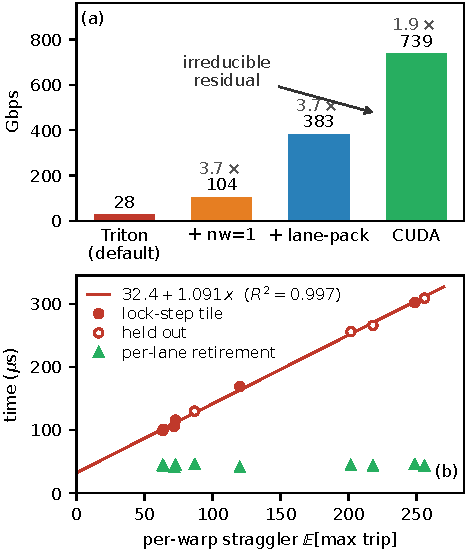
\includegraphics{figures/fig_anatomy_and_cure.pdf}
\caption{The lock-step tax, and its removal. \textbf{(a)} The NFA worklist gap
(batch 16384, $\le 64$ states) is not a monolith: a launch-configuration fix and a kernel
rewrite recover $3.7\times$ each, and an irreducible residual remains. \textbf{(b)} That
residual is the per-warp \emph{straggler} tax. Lock-step time grows linearly with
$\mathbb{E}[\max\ \mathrm{trip}]$; the line is fitted on six designed trip distributions
($R^2=0.997$) and the four open markers are held out from it. Per-lane retirement collapses
the same times to a flat, distribution-independent floor. All points oracle-gated; every number traces to a versioned CSV.}
\Description{Two stacked panels. The upper bar chart shows NFA worklist throughput rising
across four kernels, from 28 Gbps for the default Triton tile kernel to 104 after setting
num_warps to one, 383 after lane-packing, and 739 for hand-written CUDA, with an arrow
marking the final gap as the irreducible residual. The lower scatter plot shows lock-step
execution time rising linearly with the per-warp straggler across ten trip distributions,
along a fitted line, while the per-lane retirement points lie flat near 43 microseconds
regardless of the straggler.}
\label{fig:teaser}\end{figure}

This paper answers it. The gap is structural, the missing primitive can be named, and it
can be supplied inside the compiler itself.

\paragraph{One shared latch.} The mechanism is simpler than the symptom suggests. A tile
program's lanes advance in lock step under a single instruction stream, and in particular
they share one loop latch. Two consequences follow, and between them they account for the
whole residual. A data-dependent loop runs for as long as its warp's \emph{slowest} lane,
so the active lanes do full-width work the retired ones no longer need. And a
next-state load that each lane depends on cannot be overlapped with its neighbours', so
the warp cannot use its lanes as independent generators of in-flight
requests~\cite{volkov2016latency}. This is not branch or memory divergence~\cite{fung2007}:
the lanes may be perfectly coalesced and still wait together.

\paragraph{Measured, not asserted.} On the NFA worklist the gap decomposes, staged, into a
launch-configuration artifact, a redundancy that lane-packing removes, and an irreducible
residual (Fig.~\ref{fig:teaser}a). Nsight localizes that residual precisely. At matched
occupancy, issuing \emph{fewer} warp-instructions than CUDA, and sitting far below both the
issue and the bandwidth ceiling, the tile kernel spends $15.3\times$ more cycles in the
dependent-load stall. If the mechanism is latency, it should vanish when latency stops
being the binding constraint. It does: on a memory-bound DFA the residual closes once the
table spills past L2.

\paragraph{The primitive, and a wall.} The fix the diagnosis asks for is a per-lane loop
exit. TritonGPU cannot express it, and not for want of a layout: the carried tensors are
already one element per lane. \texttt{scf.condition} takes a single \texttt{i1}, so a
per-lane termination condition is rejected by the verifier. Per-lane retirement is
\emph{inexpressible} in structured tile control flow, which is a sharper statement than
``Triton is slow here'' and a falsifiable one.

\paragraph{The cure, one level down.} Since the tile IR cannot host it, we build the
primitive underneath, as an MLIR pass in \texttt{libtriton} wired into \texttt{make\_llir}.
After lowering, the per-lane predicate already exists; the lock-step latch merely
warp-reduces it away. The pass branches on the per-lane predicate instead, guarded by a
static verifier that proves observational equivalence before firing. Rebuilt from a pinned
one-command recipe, it is oracle-correct and gives $2.3$--$6.7\times$ on control-bound
kernels, $1.6$--$3.8\times$ on an A100 from the same wheel, and ${\approx}1.0\times$ on
gather-bound SpMV and MoE. That last number is not a disappointment but a prediction met:
the recoverable cost scales with per-step \emph{control}, not with memory irregularity.

\paragraph{Predictable a priori.} Finally the tax is not merely explicable after the fact.
It is set by the per-warp straggler, $\mathbb{E}[\max\ \mathrm{trip}]$, a quantity a
programmer can estimate before writing the kernel. A single-predictor fit predicts lock-step
time with $R^2=0.997$ and, with coefficients frozen, predicts four held-out distributions
to $1.5\%$ (Fig.~\ref{fig:teaser}b). The natural competing intuition, that cost tracks the
\emph{ratio} of straggler to mean, is wrong, and we falsify it.

\paragraph{Contributions.}
\begin{enumerate}
\item An instruction-level anatomy of the tile-versus-thread gap on irregular control flow,
cross-validated on two architectures, that separates what tuning recovers from an
irreducible residual and attributes the residual to abstraction-denied intra-warp latency
hiding rather than to divergence, occupancy, instruction count, or bandwidth
(\S\ref{sec:anatomy}--\S\ref{sec:mech}).
\item A structural impossibility result: per-lane loop termination cannot be expressed in
TritonGPU's tile control flow, shown by a verifier-rejected rewrite. We do not stop at
naming the missing primitive but specify it, including the body restriction it forces and
the one composition question it leaves open (\S\ref{sec:wall}).
\item That primitive, built: a soundness-verified MLIR pass in \texttt{libtriton} that
restores per-lane retirement below the tile IR, oracle-correct, reproduced on two GPUs from
one pinned wheel, and confirmed at the PTX and SASS level (\S\ref{sec:cure}).
\item A predictive model of the cost and a generality law with correct negative controls
across eight oracle-gated workloads, including a case where the sign inverts and the tile
legitimately wins (\S\ref{sec:law}--\S\ref{sec:general}).
\end{enumerate}

\section{Background and method}\label{sec:method}
NFA simulation, as a work-efficient worklist that iterates the active set with \texttt{ffs}
over a bitmask, is control-flow and latency bound. DFA simulation, one dependent table
gather \texttt{trans[cur*256+sym]} per symbol, is memory bound. Between them they give the
two faces we need. CUDA and NVIDIA Warp~\cite{warp2022} are thread-SIMT, one thread per
string; Triton~\cite{triton2019} is tile/SPMD, one program over tiles. Warp is the control
that keeps the two axes apart, because it is high-level \emph{and} thread-SIMT at once: on
this workload it reaches $0.9\times$ of hand-written CUDA. Nothing that follows is a claim
about abstraction \emph{height}.

Correctness gates speed. Every kernel and every configuration is validated bit-for-bit
against a CPU oracle before any throughput is reported, so a fast wrong kernel cannot enter
the record. We report medians over warmup${+}9$ repetitions at a GPU-saturating
batch~\cite{hoefler2015}, since GPU timings are not Gaussian; decomposition ratios are
medians over 3 seeds, with dispersion given on the load-bearing anchors. Every mechanism
claim is backed by Nsight Compute rather than wall-clock alone: issue-stall composition
(the \texttt{long\_scoreboard} reason isolates dependent-load waits), achieved occupancy,
issue activity, warp- and thread-instruction counts, and DRAM and L2 traffic.

Hardware: RTX 4070 (sm\_89, 46 SMs), Triton 3.5.1, torch 2.9.1+cu128, CUDA 13.3, driver
580; the in-\texttt{libtriton} passes (\S\ref{sec:cure}) use a from-source Triton 3.8.
Cross-architecture results are on an A100-SXM4-40GB.

\section{Anatomy of the gap}\label{sec:anatomy}

\paragraph{The anchor.} A register-resident worklist ($\le 64$ states, batch 4096, 12
configurations) gives Triton $22$\,Gbps against CUDA's $227$\,Gbps, a median of
$10.1\times$ (IQR $[9.9, 10.5]$, range $9.4$--$12.2\times$, $n{=}12$: 3 seeds $\times$ 4
state counts). The gap is batch-dependent, and reaches $26\times$ at a saturating batch as
the occupancy-gated component below saturates.

\paragraph{A: a launch-configuration artifact.} The Triton worklist defaults to
\texttt{num\_warps=4}, and four warps per program redundantly process the \emph{same}
string. Sweeping \texttt{num\_warps}$\in\{1,2,4,8\}$, \texttt{nw=1} beats \texttt{nw=4} by
$2.77\times$ at batch 4096, $3.44\times$ at 16384 and $3.69\times$ at 65536, each doubling
roughly halving throughput. The ladder of Table~\ref{tab:decomp} measures the same stage on
its own harness and lands at $3.7\times$; we quote both rather than pick the flattering
one, and take the component to be $2.8$--$3.7\times$ depending on batch. Either way this is
pure tuning, it inflates previously reported worklist gaps, and it must be disclosed rather
than absorbed into an abstraction claim.

\paragraph{B: warp redundancy, recoverable by packing.} The scalar Triton program executes
warp-uniformly. Its \texttt{thread\_inst\_per\_inst} is $32.00$ against CUDA's $30.34$: the
same number with the opposite meaning, since CUDA's 32 lanes run 32 \emph{different}
strings and Triton's run the \emph{same} one. That is ${\sim}90\times$ more
warp-instructions. Lane-packing removes it by placing 32 strings in the 32 lanes, which the
shared CSR permits because inner-loop bounds stay scalar. Pure packing recovers
$3.2\times$, $9.8\times$ and $19.4\times$ at batch 4096, 16384 and 65536, climbing toward
the ideal $32\times$ as more warps fill the device: the benefit is occupancy-gated.

We first read that $90\times$ redundancy as the bottleneck. It is not. Profiling the
lane-packed kernel shows the redundancy falls ${\sim}26\times$ while throughput moves only
$3.8\times$, because occupancy was already hiding most of it. The redundancy is real but
not load-bearing, and we report it as such.

\paragraph{C: what is left.} A per-lane Triton worklist, in which each lane runs its own
\texttt{ffs} and its own CSR gather with no cross-lane reduction and no active-set union,
beats the union variant by $1.27\times$ and still reaches only $0.51\times$ of CUDA. That
residual, ${\approx}2\times$, is the subject of the rest of the paper. Raising occupancy
does not touch it: sweeping \texttt{BLOCK}$\in\{32,64,128,256\}$ makes it \emph{worse}
($0.49\times \rightarrow 0.31\times$), because wider lock-step tiles admit more divergence.

\begin{table}[t]\centering
\caption{The staged ladder reproduces on a second architecture. Both columns are the
\emph{same} four kernels measured the same way (batch 16384, $\le 64$ states, medians over
seeds and state counts, every row oracle-gated), so the stages are comparable across
devices. The total is architecture-stable; the split between the last two stages is not.
Fig.~\ref{fig:teaser}a shows the sharper per-lane lane-packed variant, which reaches
$383$\,Gbps but was measured on the 4070 only.}
\label{tab:decomp}
\small
\begin{tabular}{@{}lrrrr@{}}
\toprule
& \multicolumn{2}{c}{RTX 4070} & \multicolumn{2}{c}{A100} \\
\cmidrule(lr){2-3}\cmidrule(l){4-5}
Kernel & Gbps & stage & Gbps & stage \\
\midrule
Triton worklist (\texttt{nw=4}) & 28 & --- & 28 & --- \\
\quad $+$ \texttt{nw=1} & 104 & $3.7\times$ & 101 & $3.7\times$ \\
\quad $+$ lane-packing & 314 & $3.0\times$ & 233 & $2.3\times$ \\
CUDA worklist (thread-SIMT) & 739 & $2.4\times$ & 705 & $3.0\times$ \\
\midrule
total & & $\mathbf{26\times}$ & & $\mathbf{25\times}$ \\
\bottomrule
\end{tabular}
\end{table}

Table~\ref{tab:decomp} puts the three components together and repeats the whole ladder on
an A100. The total is architecture-stable, $26\times$ against $25\times$, and the
launch-configuration stage is identical on both devices. The remaining two stages trade
places, $3.0\times$ then $2.4\times$ on the 4070 against $2.3\times$ then $3.0\times$ on
the A100, which is what one expects when the A100's larger L2 and lower clock move where
the occupancy-gated benefit saturates. What does not move is that the ladder ends with a
stage the tile model cannot climb.

\section{The mechanism}\label{sec:mech}

\begin{figure*}[t]\centering
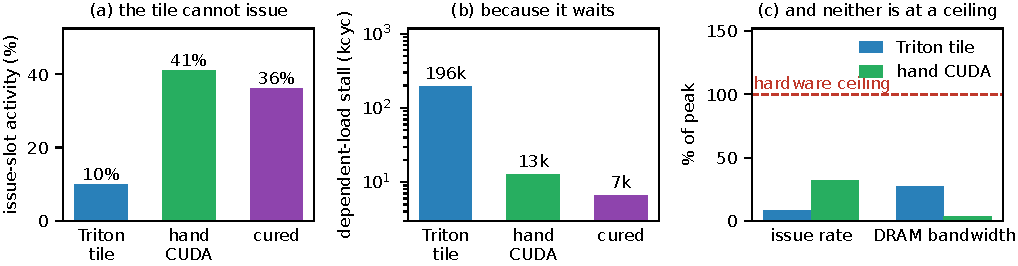
\includegraphics{figures/fig_mechanism.pdf}
\caption{Why the residual is latency and not something cheaper to fix (32 states, batch
16384). \textbf{(a)} The per-lane tile kernel occupies its issue slots a quarter as often
as CUDA, and per-lane retirement restores it. \textbf{(b)} The missing time is the
dependent-load stall (\texttt{long\_scoreboard}), $15.3\times$ CUDA's on the tile and
$29\times$ lower again once cured. \textbf{(c)} Neither kernel is near a hardware ceiling,
so this is not a worse kernel: it is a kernel that cannot keep loads in flight.}
\Description{Three bar panels comparing the Triton tile kernel, hand-written CUDA and the
cured kernel. The first shows issue-slot activity of 10 percent for the tile against 41
percent for CUDA and 36 percent once cured. The second, on a logarithmic axis, shows the
dependent-load stall at 196 thousand cycles for the tile, 13 thousand for CUDA and 7
thousand cured. The third shows both kernels far below the hardware ceiling on issue rate
and on DRAM bandwidth.}
\label{fig:mech}\end{figure*}

Fig.~\ref{fig:mech} settles what the residual is. In the profiled configuration the
per-lane tile kernel issues \emph{fewer} warp-instructions than CUDA ($4.66$M vs.\
$5.07$M) at the same occupancy ($22.5\%$), and is nonetheless $3.3\times$ slower.\footnote{%
The $0.51\times$ of \S\ref{sec:anatomy} is the median head-to-head across the $\le
64$-state sweep; $3.3\times$ is this specific Nsight-profiled configuration. The residual we
attribute is the ${\sim}2\times$.} Its issue activity is $9.9\%$ against CUDA's $41\%$, and
it spends $15.3\times$ more cycles waiting on a dependent load. The issue-rate ratio
($4.1\times$) tracks the throughput ratio ($3.5\times$), which is what Little's law predicts
when latency is fixed and concurrency is the free variable~\cite{volkov2016latency,hongkim2009}.

The instruction roofline~\cite{instroofline2022} closes the obvious objection, that we
simply wrote a worse kernel. Both kernels sit far below the issue \emph{and} the
bandwidth ceiling ($8.3\%/27\%$ for Triton, $32\%/3.4\%$ for CUDA). A kernel that is
neither instruction- nor bandwidth-bound, issues fewer instructions than its rival, and
still runs $3.5\times$ slower, is latency-bound by elimination.

One refinement runs against our own initial reading. We predicted, following the
latency-hiding literature, that the tile kernel would sustain \emph{fewer} in-flight
requests. It sustains $26$--$84\times$ \emph{more}, because inactive lanes still issue
masked gathers. So the tile pays twice, in excess masked traffic and in an inability to
overlap the dependent load, and the mechanism must be stated through stall composition and
issue activity rather than request counts.

We also distinguish this from the hardware fix for intra-warp stalls~\cite{subwarp2022}.
The same SM is fast under CUDA and slow under Triton at equal occupancy and fewer
instructions, so the loss is imposed by the abstraction, not by the machine.

\paragraph{The regime test.} A latency explanation makes a falsifiable prediction: where
latency is not the binding constraint, the residual should vanish. The DFA supplies the
test. Across table sizes the scalar Triton DFA is flat at ${\sim}29$\,Gbps, an independent
confirmation of the scalar-gather ceiling, and lane-packing gives ${\sim}12\times$ over it.
The lane-packed-to-CUDA ratio is $0.55$--$0.62\times$ while the table is cache-resident but
$1.05\times$ at a $16$\,MB table (Fig.~\ref{fig:dfa}): lane-packed Triton \emph{matches}
CUDA. DRAM utilization is only $14.6\%$ there, so this is memory \emph{latency}, not
saturated bandwidth. At cache latency CUDA's intra-warp hiding wins ${\sim}1.7\times$; at
DRAM latency both must hide latency across warps, and they converge. The NFA's irreducible
residual and the DFA's closeable gap are one mechanism at two latency scales.

\begin{figure}[t]\centering
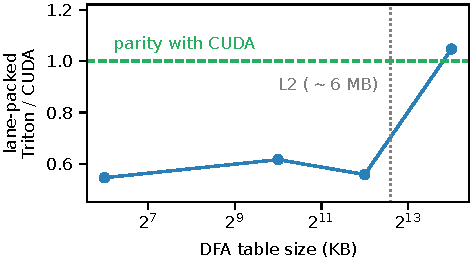
\includegraphics{figures/fig_dfa_crossover.pdf}
\caption{The residual is regime-dependent. Lane-packed Triton trails CUDA by ${\sim}1.7\times$
while the DFA table is cache-resident and reaches parity ($1.05\times$) once a $16$\,MB
table spills past L2, where both must hide latency across warps.}
\Description{A line chart of the ratio of lane-packed Triton throughput to CUDA throughput
against DFA table size on a logarithmic axis. The ratio sits between 0.55 and 0.62 while
the table is cache-resident and rises to 1.05, crossing the parity line, once the table
exceeds the roughly six megabyte L2.}
\label{fig:dfa}\end{figure}

\section{The wall: per-lane exit is inexpressible}\label{sec:wall}

The diagnosis names what a fix must provide: independent per-lane \texttt{ffs} and
\texttt{while}, per-lane data-dependent loop bounds, a register-resident per-lane bitset,
and a scalar gather. Call it a per-lane sub-tile loop with an independent exit. The
natural place to add it is the tile IR. It cannot go there, and showing why is the
sharpest result in this paper because it is a statement about the abstraction rather than
about one compiler's maturity.

We first checked whether a lower-level tile frontend already supplies it. It does not.
Triton's Gluon exposes per-thread \emph{layout} through Linear
Layouts~\cite{linearlayouts2025}, not per-lane \emph{control flow}: a runnable probe shows
\texttt{gl.load} returns a layout-typed block and never a scalar, so the data-dependent CSR
loop cannot be lowered at all, and we capture the compile error verbatim. Layout control is
not control-flow divergence.

Two facts from the matched TritonGPU IR then close the question.

\begin{figure}[t]
\footnotesize
\begin{verbatim}
#blocked = <{sizePerThread = [1],   // already ONE
             threadsPerWarp = [32]}>  // element/lane

%j:2 = scf.while (%acc = %cst, %j = %cst) : (
    tensor<32xi32, #blocked>, ...) -> (...) {
  %2 = arith.cmpi slt, %j, %trip
     : tensor<32xi32, #blocked>   // per-lane predicate
  %5 = "tt.reduce"(%2) <{axis = 0}>  // ...destroyed here
     : (tensor<32xi32, #blocked>) -> i32
  %6 = arith.cmpi sgt, %5, %c0 : i32
  scf.condition(%6) %acc, %j : ...  // ONE i1, 32 lanes
} do {                     // masked full-width body
  %active = arith.cmpi slt, %j, %trip
  %acc_9  = arith.select %active, %j, %cst
  ...
}
\end{verbatim}
\caption{The lock-step latch, in the matched TritonGPU IR (trimmed; source locations
removed). The lanes already hold one element each, so no layout change can help. The
per-lane predicate \texttt{\%2} exists and is then reduced to a scalar, because
\texttt{scf.condition} admits exactly one \texttt{i1} for the whole tile. That single
\texttt{i1} is the lock-step.}
\Description{A trimmed listing of TritonGPU intermediate representation. The blocked layout
declares one element per thread. Inside an scf.while loop an arith.cmpi computes a per-lane
predicate over a 32-element tensor, a tt.reduce collapses it to a single i32, a comparison
turns that into one i1, and scf.condition consumes that single i1 for the whole tile. The
loop body then does masked full-width work.}
\label{fig:ir}
\end{figure}

\emph{The lock-step is not a layout choice.} The tensors carried by the loop are already
\texttt{sizePerThread=1}, one element per lane. Re-encoding them is a no-op, so no amount
of per-thread layout, in Gluon or anywhere else, changes the behaviour.

\emph{The lock-step is the loop construct itself.} Fig.~\ref{fig:ir} shows where. The
per-lane predicate is computed and then immediately destroyed: a \texttt{tt.reduce}
collapses the 32-lane comparison to one \texttt{i32}, and \texttt{scf.condition} consumes
a single \texttt{i1}. The natural rewrite is to carry the per-lane condition instead, and
the MLIR verifier rejects it on the type
(\emph{``'i1' vs 'tensor}$\langle$\emph{8}$\times$\emph{i1}$\rangle$\emph{'''},
captured with the built \texttt{triton-opt}). Per-lane loop termination is therefore
\emph{inexpressible} in TritonGPU's structured tile control flow.

That is falsifiable and it is actionable. It is falsifiable because adding a per-lane
sub-tile loop and exit op to the tile IR would make the statement false, which is precisely
the language change we are arguing for. It is actionable because it tells us where the cure
has to live: below the tile IR, in the lowering to the thread model.

\paragraph{What the primitive would have to be.} Naming a missing op is cheap unless one
says what it must mean, so here is the specification our lowering already implies. Take
\texttt{scf.while}'s condition from \texttt{i1} to a tile of \texttt{i1} under the same
layout as the carried tensors, and read it lane-wise: a lane whose predicate is false takes
no further trips and stops updating its slice of the iter-args, and the region exits when
no lane is still live. Live-outs freeze, per lane, at the trip on which that lane left.
That freezing is what makes the construct observationally equivalent to today's masked
loop, rather than merely faster than it.

The price is a restriction on the body, and it is not incidental. A retired lane cannot
participate in a cross-lane operation, so the region may not contain reductions,
broadcasts, or tile-wide shared-memory operations. That is exactly the body-safety
condition our verifier already discharges (\S\ref{sec:cure}), so the analysis a compiler
would need in order to admit the op is one we have had to write anyway. Reconvergence for
whatever tile operation follows is a barrier at the join, which is the
\texttt{bar.warp.sync} our pass inserts.

What stays genuinely open is composition with tile operations that assume full width,
\texttt{tt.dot} above all. The op is an escape hatch for scalar control and has no business
inside a matmul, so the question is where a language draws that boundary, not whether the
lowering works.

\section{Per-lane retirement, built}\label{sec:cure}

\subsection{Detecting the region}
On a from-source Triton (3.8.0) we add a TritonGPU pass, \texttt{tritongpu-thread-region},
that runs in the NVIDIA \texttt{make\_ttgir} pipeline and recognises the lock-step
signature: an \texttt{scf.while} whose iter-args are \texttt{\#blocked} tile tensors and
whose \texttt{scf.condition} derives from a \texttt{tt.reduce} to scalar, which is exactly
``the whole tile loops until the busiest lane is done, and idle lanes are masked''. It
compiles into \texttt{libtriton} and fires on the target kernels; with the pass off the
attribute is absent and codegen stays bit-exact.

\subsection{What can be fixed inside the tile IR, and what cannot}
Part of the cost is reachable without leaving the tile IR. The per-iteration
\texttt{tt.reduce} that gates the lock-step \texttt{while} is loop-invariant in disguise:
the lane counter is a uniform splat, so \texttt{any}$(j<\mathit{trip})$ equals
$j<\max(\mathit{trip})$. We extend the pass, behind a flag, to hoist
\texttt{reduce\_max(trip)} once before the loop and replace the per-iteration cross-lane
reduce with a scalar counter, leaving the masked body untouched. It is provably
equivalent, preserves per-warp termination, is verified bit-exact end-to-end, and is
$1.55\times$ faster on the lock-step kernel ($155.6\rightarrow100.4\,\mu$s; detection-only
mode is a performance no-op, which confirms the gain is the rewrite and not the pass
machinery).

This is an honest partial. It removes the reduce overhead. It does not grant per-lane
retirement, because \S\ref{sec:wall} says it cannot.

\subsection{The full primitive, below the tile IR}
After \texttt{convert-triton-gpu-to-llvm} the per-lane predicate already exists as a scalar
$j_{\mathrm{lane}}<\mathit{trip}_{\mathrm{lane}}$, and the lock-step latch merely
warp-reduces it (\texttt{nvvm.redux.sync}) into a uniform \texttt{i1} that gates
\texttt{llvm.cond\_br}. That is the whole lock-step, in one instruction, at a level where
we can reach it.

Our pass, a real MLIR pass in \texttt{libtriton} wired into \texttt{make\_llir}, redirects
the branch to the per-lane predicate so each lane retires independently under hardware
Independent Thread Scheduling~\cite{its2017}, deletes the now-dead cross-lane reduce, and
inserts a \texttt{bar.warp.sync} at the reconvergence block.

The rewrite is visible all the way down. In PTX the masked baseline reduces the active mask
(\texttt{redux.sync.max.s32}) and branches the warp on the resulting uniform predicate,
whereas the cured code branches on this lane's own \texttt{setp.lt.s32} and carries a
\texttt{bar.warp.sync} at reconvergence (\texttt{redux.sync} $1\!\rightarrow\!0$,
\texttt{bar.warp.sync} $0\!\rightarrow\!1$). It survives \texttt{ptxas} to SASS: the
warp-collective \texttt{REDUX.MAX.S32} into a uniform register disappears
(\texttt{REDUX} $1\!\rightarrow\!0$, static instructions $48\!\rightarrow\!40$) and the
latch branches on the per-lane \texttt{ISETP}, with reconvergence realized by the standard
\texttt{BSSY}/\texttt{BSYNC} barriers. Per-lane retirement is in the machine code, not only
in the IR.

\subsection{Sound by default}
A rewrite that changes when lanes stop executing is only safe under conditions we can
check, so the pass fires only behind a static verifier that proves observational
equivalence: body safety (no cross-lane op anywhere in the loop body), a single exit,
live-out freezing through the lowering's struct projections, and predicate
\emph{monotonicity}, which live-out freezing alone does not imply. Where the proof fails,
the pass declines.

That is not hypothetical. On a rejection-sampling kernel whose latch is an accumulate-OR
early exit rather than a counter-versus-bound compare, the verifier cannot establish
monotonicity and declines to fire, on both GPUs, leaving the kernel bit-exact
(Table~\ref{tab:builtcure}). We would rather report a decline than a rewrite we cannot
justify.

\subsection{What it recovers}
Compiled and run end-to-end from a pinned recipe (a base commit plus a versioned patch,
built to a wheel), the pass is oracle-correct and gives $2.3$--$6.7\times$ across six trip
distributions on the RTX 4070 (geometric law: median $2.46\times$, IQR $[2.46,2.50]$,
$n{=}5$ seeds) and $1.6$--$3.8\times$ on an A100 from the \emph{same} wheel. On both GPUs
the cured time collapses to a flat, distribution-independent floor ($43.0\pm1.6\,\mu$s and
${\sim}75\,\mu$s), which is the mechanism's signature: once each lane retires at its own
trip count, the distribution stops mattering.

These six are a synthetic kernel with injected trip divergence. They isolate the mechanism
and \emph{upper-bound} the payoff; they are not a general speedup claim. Nsight attributes
the gain to work, not occupancy: issued instructions fall $39\times$
($36.1\mathrm{M}\rightarrow0.92\mathrm{M}$) because total work becomes
$\sum_i \mathit{trip}_i$ rather than $32\times$ the busiest lane, while
threads-per-instruction is unchanged.

\paragraph{Which cost this closes, and which it does not.} The residual of \S\ref{sec:mech}
and the tax of \S\ref{sec:law} are both consequences of the shared latch, but they are not
the same cost, and it matters that the pass addresses one of them. Per-lane retirement
removes the work the lock-step forces on lanes that should already have stopped, which is
why Nsight reports its gain as instructions rather than as stall cycles. Restoring the
intra-warp latency hiding of \S\ref{sec:mech} additionally requires the lanes to be running
independent work, which is what the thread lowering below does and what the tile IR
withholds for the same structural reason as \S\ref{sec:wall}. We measured each with the
metric that applies to it, and we do not claim the pass was shown to do the other's job.

The pass also fires, oracle-correct, on real workloads carrying the same latch: power-law
CSR SpMV and MoE top-$k$ routing, with \texttt{redux.sync} removed and
\texttt{bar.warp.sync} present in the emitted PTX. Both carry a per-iteration memory
gather, so almost none of their cost is the control reduce, and the gain is
correspondingly ${\approx}1.0\times$ on both GPUs. We report this as the honest end-to-end
value, and as a confirmation rather than a failure: that the \emph{same} pass yields
$2.3$--$6.7\times$ on control-bound work and nothing on gather-bound work is the thesis,
measured.

\begin{table}[t]\centering
\caption{The built pass, rebuilt from one pinned wheel and run on two GPUs. Speedup is
against the masked tile baseline; every row is oracle-correct, and every row traces to a
versioned CSV. The benefit scales with control-boundedness, and the verifier declines the
out-of-scope latch rather than rewriting it.}
\label{tab:builtcure}
\small
\begin{tabular}{@{}llrr@{}}
\toprule
Workload & Bound by & RTX 4070 & A100 \\
\midrule
Lock-step \texttt{while} (6 dists) & control & $\mathbf{2.3}$--$\mathbf{6.7\times}$ & $1.6$--$3.8\times$ \\
\quad geometric ($n{=}5$ seeds) & control & $2.46\times$ & $1.8\times$ \\
\quad single-straggler (held out) & control & $7.2\times$ & n/a \\
MoE top-$k$ routing & gather & ${\approx}1.0\times$ & ${\approx}1.0\times$ \\
SpMV CSR (power-law) & gather & ${\approx}1.0\times$ & ${\approx}1.0\times$ \\
Rejection sampling & control & \emph{declines} & \emph{declines} \\
\bottomrule
\end{tabular}
\end{table}

\subsection{An out-of-band bound, and the loop closed}
Two results sit beside the in-compiler pass, and which is which matters.

\emph{The bound.} Out of band, we lower the \emph{same} idiomatic per-lane source, the
active-set \texttt{ffs} worklist with its data-dependent CSR loop, to a per-thread CUDA
kernel through \texttt{nvcc}. Oracle-validated on no-accept automata, which removes the
early-exit confound, that lowering runs $4.2\times$ the tile lowering (${\approx}1555$
vs.\ ${\approx}378$\,Gbps) and exceeds hand-written CUDA ($2.15\times$, the generated
kernel being a minimal thread worklist). It is an existence proof and an upper bound, not
the contribution: the front-end source was never the problem, the tile lowering is. The
second number cuts our way and we would rather state it than let it be found: our hand-CUDA
baseline is evidently not the thread model's ceiling, so every gap this paper reports
against it is a \emph{lower} bound on what the tile lowering forgoes. It also
acts through the diagnosed mechanism, restoring issue activity to $36\%$ against the tile's
$9.9\%$ and CUDA's $41\%$ and cutting the dependent-load stall $29\times$
(Fig.~\ref{fig:mech}).

\emph{The loop.} A selector then closes the pipeline. It runs the detection pass of
\S\ref{sec:cure}, and where the lock-step signature is present routes the region to
\emph{that out-of-band lowering}, otherwise leaving it on the tile path. Oracle-gated, the
NFA worklist is auto-routed for $3.9\times$ over the tile across a $16$--$64$ state sweep,
consistent with the $4.2\times$ above, while a fixed-trip negative control is
detected-negative and stays on the tile path. Detect, decide, lower, measured, end to end.

We are explicit about the seam. The detection is a pass inside \texttt{libtriton}; the
lowering the selector routes to is not, and we have not wired the selector to the in-IR
per-lane-retirement pass of \S\ref{sec:cure}. The two halves of the loop are each real and
each measured, and joining them inside the compiler is engineering we have not done.

\section{The tax is the straggler}\label{sec:law}

\begin{figure}[t]\centering
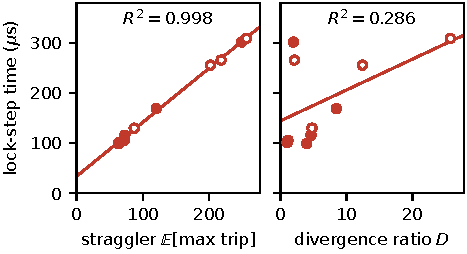
\includegraphics{figures/fig_straggler_law.pdf}
\caption{The lock-step cost is set by the absolute straggler, not by the divergence
\emph{ratio}. Ten trip distributions, filled markers designed, open markers held out.
A linear fit on the straggler alone explains the cost; the same fit on
$D=\mathbb{E}[\max\ \mathrm{trip}]/\mathbb{E}[\mathit{trip}]$ does not.}
\Description{Two scatter panels of lock-step time against two candidate predictors over the
same ten trip distributions. Against the per-warp straggler the points lie tightly along a
fitted line with an R-squared of 0.998. Against the divergence ratio they form a scattered
cloud with an R-squared of 0.286.}
\label{fig:straggler}\end{figure}

A diagnosis is worth more if it predicts. A controlled sweep over six trip distributions
(constant, low-variance, wide-uniform, geometric, and two Pareto laws; $2^{20}$ elements
each, oracle-gated in both modes) pins the masked baseline to a single \emph{a-priori}
quantity, the per-warp straggler $\mathbb{E}[\max_{\mathrm{warp}}\mathit{trip}]$. Least
squares gives
\[
t_{\mathrm{masked}} = 32.4 + 1.09\;\mathbb{E}[\text{warp-max}]\;\mu\text{s},
\qquad R^2 = 0.997,
\]
which is what a latch that iterates to the busiest lane must do. The cured kernel collapses
to the flat floor of \S\ref{sec:cure} because each lane retires at its own trip count. The
slope is the kernel's per-iteration lock-step cost and the intercept is compiler
overhead.

\paragraph{The intuitive predictor is the wrong one.} It is natural to expect the cost to
track the intra-warp divergence \emph{ratio}
$D=\mathbb{E}[\text{warp-max}]/\mathbb{E}[\mathit{trip}]$. It does not.
Fitting the same masked times against $D$ gives $R^2=0.00$ over the six designed
distributions and only $0.29$ once the four held-out ones are added, against $0.997$ and
$0.998$ for the straggler on the same two samples (Fig.~\ref{fig:straggler}). The concrete
inversion makes the point: the geometric law ($D=3.96$) yields $2.3\times$ while
wide-uniform ($D=1.94$) yields $6.7\times$, a \emph{lower} ratio but a much larger absolute
straggler, hence more lock-step waste. What is wasted is warp-cycles, and warp-cycles are
counted in absolute iterations.

\paragraph{Out of sample.} With the coefficients frozen, the model predicts four
\emph{held-out} distributions generated from a different seed (bimodal, log-normal, spike,
and an adversarial single-straggler warp in which $1/32$ lanes run $256$ iterations and the rest
run $2$) to within $1.5\%$ on average and $2.1\%$ at worst on lock-step time, and every
in-sample speedup to under $8\%$. That last case yields $7.2\times$, the effect at its
purest: one slow lane taxing the other $31$, which is what per-lane retirement removes.

\paragraph{What the law is, and is not.} The validation is across trip
\emph{distributions} of one kernel, not across kernels, and the two coefficients are that
kernel's own: change the loop body and both move. What transfers is the \emph{form}, that
cost follows the absolute straggler rather than the divergence ratio, and two things
support it beyond one good fit. The coefficients are not free parameters but have a
mechanical reading, and the slope survived a rebuild of the pass that moved the intercept
($1.08$ against $1.09$, intercept $50\rightarrow32\,\mu$s). So a programmer gets the right
\emph{shape} of estimate before writing a kernel and calibrates the constant on their own
body, which is still better than the qualitative ``divergent trips cost more'' it
replaces.

\section{Generality, and where it stops}\label{sec:general}

\begin{figure*}[t]\centering
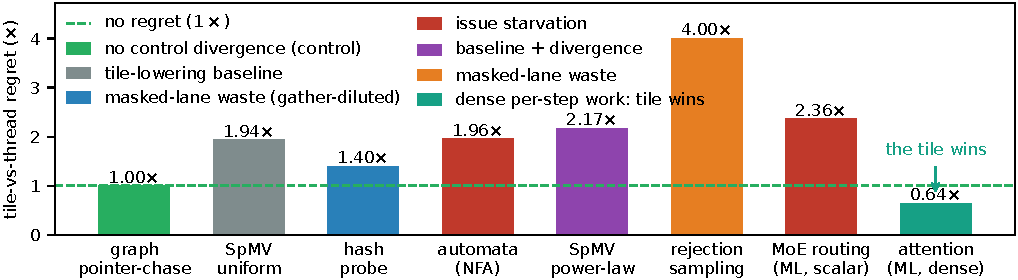
\includegraphics{figures/fig_regret_law.pdf}
\caption{Tile-versus-thread regret across eight oracle-gated irregular witnesses, coloured
by dominant mechanism. The graph pointer-chase is the negative control: irregular memory
and dependent loads with a \emph{fixed} step count cost nothing at all. Uniform SpMV is the
other half of the story: no divergence either, but the tile mapping loses occupancy, so a
floor can exist without any control cost. What grows \emph{above} such a floor is set by
per-step scalar control. Ragged attention inverts the sign, because a dense head-dim payload makes
the tile issue \emph{fewer} instructions than the thread model.}
\Description{A bar chart of tile-versus-thread regret across eight workloads, coloured by
dominant mechanism. The graph pointer-chase sits exactly at the no-regret line at 1.00
times. Uniform SpMV is 1.94, hash probe 1.40, automata 1.96, power-law SpMV 2.17, MoE
routing 2.36 and rejection sampling 4.00. Ragged attention alone falls below the no-regret
line at 0.64 times, where the tile wins.}
\label{fig:law}\end{figure*}

Is any of this specific to automata? To find out we built six further oracle-gated
tile-versus-thread witnesses spanning the irregularity space, each with identical machinery
(a Triton tile kernel, the same per-lane source lowered to CUDA threads, and a CPU oracle),
and then two more drawn from ML. Fig.~\ref{fig:law} reports the result. The law is that
\textbf{the regret that grows, and that the cure recovers, is created by per-step scalar
control rather than by memory irregularity}. It is deliberately not the stronger claim that
all regret is, because a tile mapping can also lose occupancy and charge a floor with no
divergence anywhere, which we measure below.

\paragraph{The negative control.} A graph pointer-chase, one million random walkers with
data-dependent gather addresses over scattered \texttt{colidx} at degree CV $3.79$, but a
\emph{fixed} step count, is the decisive case. Tile and thread are indistinguishable in
issue activity ($5.42\%$ vs.\ $5.43\%$), occupancy ($72.1\%$ vs.\ $72.1\%$) and
threads-per-instruction ($32$ vs.\ $32$), and the regret is $1.00\times$. Irregular memory
and dependent loads on their own cost nothing, because a lock-step gather already supplies
full intra-warp memory-level parallelism.

\paragraph{Two channels, not one.} We first stated the law as a single ``tile issue
deficit'' predictor. Completing the Nsight profiling falsified that, and the honest form has
two channels. \emph{Issue starvation}: a data-dependent scalar recurrence drives the tile's
issue rate below the thread's, as in the NFA worklist ($1.96\times$ at $9.9\%$ vs.\ $41\%$).
\emph{Masked-lane waste}: divergent trip counts make the tile do full-width work where the
thread retires lanes, as in rejection sampling ($4.0\times$, tile threads-per-instruction
$32$ against the thread's $17$) whose issue rate is if anything \emph{above} the thread's,
so the waste is in what the active lanes compute. The floor is the third component, and it is
divergence-free: uniform-\texttt{nnz} SpMV has zero divergence and still costs
$1.94\times$, because the tile mapping loses occupancy against the thread mapping on a
bandwidth-bound gather. It is not universal, since the pointer-chase pays no floor at
matched occupancy, but it is real where the mapping costs occupancy. That falsified our
initial guess that it would be ${\approx}1\times$, and it is why the law above is scoped
to the regret that \emph{grows}. Divergence then adds on top of the floor, taking power-law
SpMV from $2.17\times$ at tile width $32$ to $5.8\times$ at $256$. So the law is
multi-component, and only its variable part is what per-lane retirement can return.

\paragraph{It reaches ML, including where it reverses.} Two witnesses on the kernels tile
DSLs are actually built for. \emph{MoE top-$k$ routing}, with ragged data-dependent expert
counts and a scalar per-token accumulate, is the ML face of scalar control: regret
$2.36\times$, the tile issuing $2.6\times$ more instructions ($41.8$M vs.\ $16.3$M) and
doing masked full-width work (threads-per-instruction $30.1$ vs.\ $7.7$).
\emph{Ragged variable-context attention} has the \emph{identical} ragged structure but a
\emph{dense} head-dim payload per step, and here the law predicts a \emph{negative} and is
right: regret $0.64\times$, the tile wins. The thread model retires lanes in both cases
(threads-per-instruction $3.45$ on attention against $7.7$ on MoE); what flips the sign is
per-step instruction efficiency. Scalar work makes the tile issue
more, through the lock-step reduce and masking, so it loses; a dense vectorizable head-dim
makes it issue fewer ($123$M vs.\ $178$M) so it wins despite no lane retirement.

That is why Triton is the tool of choice for flash-attention and collapses on automata, and
it is a scope statement as much as a generalization. These witnesses use the framework's
one-element-per-lane mapping; production attention is warp-cooperative, a different design
point, and whether the law survives there is future work.

\section{Threats to validity}\label{sec:threats}

\paragraph{One GPU, mostly.} The primary results are on an RTX 4070. The \emph{mechanism}
is a property of the SIMT execution model and the tile-versus-thread lowering rather than
of a device, so we test it directly: a one-command harness re-runs every witness on a new
GPU, tags output by device, and checks the falsifiable prediction that each regret persists
in \emph{direction} while magnitudes rescale. On an A100-SXM4-40GB (sm\_80, $6.7\times$ the
L2) all five portable witnesses confirm it with genuinely re-measured, architecture-different
magnitudes, from hash-probe ($1.40\!\to\!1.48$) to power-law SpMV
($2.17\!\to\!3.20$), while the memory-only control stays paradigm-neutral
($0.99\!\to\!0.99$). The flagship ladder reproduces too
(Table~\ref{tab:decomp}), as does the built pass (Table~\ref{tab:builtcure}). We report
the ladder's stage factors from the two devices' own measurements rather than asserting
they match: the total holds to within $3\%$ while the internal split shifts, and that is
the honest form of the claim. The
batch-4096 anchor rescales $10.1\times\!\to\!5.6\times$, because that register-resident
regime is clock-sensitive and the A100's lower clock compresses both sides; the direction
persists.

\paragraph{Where the pass applies.} The lowering is a real MLIR pass in \texttt{libtriton},
but it fires only on the \texttt{tl.max} lock-step latch, and the body-safety guard bails
when the loop carries a cross-lane op. That the cure must live below the tile IR is a
property of \emph{today's} tile IR, and \S\ref{sec:wall} states exactly the language change
that would move it up.

\paragraph{Regime of the clean residual.} A multi-word generalization of the lane-packed
kernel (NWORDS int64 words per lane) is oracle-validated to 256 states, so the prototype is
not artificially small. But the clean ${\sim}2\times$ residual is a register-resident
($\le 64$-state) result. Past 64 states the CUDA register worklist itself degrades under
register pressure, so the head-to-head is confounded by \emph{both} baselines losing the
register-resident advantage, and ANMLZoo-scale automata (Brill, 42661 states, 667 words)
make the per-lane multi-word scatter explode, which is itself a manifestation of the tile
limitation. Real automata run oracle-valid but sub-Gbps, an \emph{algorithmic} cost
orthogonal to the regret.

\paragraph{Tuning, not expressibility.} \texttt{num\_warps} is a knob, and the strongest
counter-thesis is that this is all under-tuning~\cite{ringlein2025}. We disclose the full
sweep rather than one configuration, which separates the two: tuning closes component A and
part of B, while the residual C is flat across the sweep. The Triton/Gluon pair adds a
control with the same MLIR stack in which only the expressivity lever moves, and
\S\ref{sec:wall} converts the claim into a verifier-checkable statement rather than a
judgement call.

\paragraph{On our own corrections.} Three intermediate hypotheses of ours were wrong and we
report them where they arose rather than in a footnote: warp redundancy as the bottleneck
(\S\ref{sec:anatomy}), a request-count deficit as the mechanism (\S\ref{sec:mech}), and a
single-channel issue-deficit law (\S\ref{sec:general}); a fourth, that uniform SpMV would
show ${\approx}1\times$, was falsified at $1.9\times$. Each correction narrowed the claim,
and we prefer that record to a cleaner-looking one.

\section{Reproducibility}\label{sec:repro}
Every number here traces to a versioned CSV, and all figures regenerate from those CSVs
through a single script, so plots cannot drift from measurements. An artifact index maps
each claim to the command that produces it and the CSV it writes.

The expressibility and structural claims are \emph{runnable, falsifiable probes} rather than
prose. The Gluon probe exits $0$ on the expected compile failure and $1$ if some future
Gluon compiles it; the lowering-wall probe asserts that the MLIR verifier rejects a per-lane
\texttt{scf.condition}; the detection check confirms the pass tags the lock-step region with
the flag set and is a no-op without it. The per-lane-retirement pass builds as a wheel from
a one-command recipe (a pinned upstream commit plus a versioned patch), and every cure
number here came from that wheel, on both GPUs. The cross-architecture re-validation is a
single non-mutating command.

\section{Related work}\label{sec:related}
\textbf{GPU automata} form an \emph{algorithmic} axis, all single-implementation CUDA:
ngAP's non-blocking multi-symbol processing~\cite{ngap2024}, HybridSA's bit-parallel
shift-and~\cite{hybridsa2024}, BitGen's Parabix bitstreams~\cite{bitgen2025}, AsyncAP's
input-symbol asynchrony~\cite{asyncap2023}, AutomataBLAS's AP-as-SpMV~\cite{automatablas2025},
and the Hopps sparsity ASIC~\cite{hopps2025}. Each varies the algorithm on one
implementation; none compares programming models or holds the algorithm fixed across them.
The sole IR-for-automata work~\cite{mlirregex2025} lowers regex to one fixed
domain-specific accelerator, a hardware target rather than a GPU-paradigm study, with no
tile-versus-thread cost. Our axis is orthogonal: fixed algorithm, varied programming model.

\textbf{Tile GPU DSLs.} Triton~\cite{triton2019} and the 2024--26 wave exposing more
thread and warp control. The closest, Gluon's Linear Layouts~\cite{linearlayouts2025},
gives per-thread \emph{data placement} but not per-lane \emph{control flow}, as our probe
shows; Descend~\cite{descend2024} makes the thread hierarchy first-class but offers no tile
drop-to-scalar escape; Warp~\cite{warp2022} is the thread-SIMT existence proof.
ML-Triton~\cite{mltriton2025} is the clearest sign of the trend and of its stopping point:
it moves Triton's interface one level finer, adding warp-level programming and a
workgroup$\rightarrow$warp$\rightarrow$intrinsic lowering, and reaches $95\%$ of
expert-written kernels on dense GEMM and attention. A warp is still $32$ lanes under one
latch, so it halts exactly one level above where the cost we measure lives.

\textbf{Mixing thread- and tile-level execution} is the live frontier, and every approach
is programmer-directed or differently directed. Prism~\cite{prism2026} makes thread
granularity part of the type system so group-coordinated code composes safely, but the
granularity is still the one the programmer writes, and nothing diagnoses that an existing
tile kernel is paying a lock-step tax. NVIDIA's cuTile~\cite{cutile2025} and its MLIR Tile
IR, now being built as a Triton backend, is tile-level and concedes the irregular case to a
hand-written SIMT fallback, so the per-lane gap we name persists in \emph{both} TritonGPU
and Tile IR; the primitive we propose is complementary to that direction rather than
subsumed by it. Tawa~\cite{tawa2026} auto-restructures Triton but for \emph{dense} warp
specialization. Partial control-flow linearization~\cite{partialcfg2018} runs the
\emph{opposite} way, vectorizing divergent CPU control flow, where we de-vectorize a tile
region to recover per-lane memory-level parallelism. None automatically detects an
irregular data-dependent per-lane region in a tile DSL and lowers it to the thread model,
and our structural result says why an in-tile-IR rewrite cannot suffice.

\textbf{Mechanism.} We ground the residual in latency-hiding and MLP-versus-occupancy
analysis~\cite{volkov2016latency,hongkim2009} and place both kernels on the instruction
roofline~\cite{instroofline2022}; we distinguish it from divergence~\cite{fung2007} and
from the \emph{hardware} fix of Subwarp Interleaving~\cite{subwarp2022}, attributing the
same stall to the DSL at equal occupancy and fewer instructions. Compiler work on
divergence reduces it by melding similar control flow~\cite{darm2022} or by linearizing
it~\cite{partialcfg2018}; both keep one instruction stream per warp, where we hand the
lanes their own.

\textbf{Methodology and lineage.} Rigorous benchmarking~\cite{hoefler2015},
roofline~\cite{roofline2009}, and the performance-portability metric~\cite{pennycook2016},
which is per-hardware where we measure per-\emph{capability}; we answer the autotuning
counter-thesis~\cite{ringlein2025} with the same-MLIR control and the disclosed sweep. The
gap we fill is a constructive, instruction-level account of \emph{why} a tile DSL pays on
irregular control flow, which names the missing primitive and builds it.

\section{Conclusion}
The cost a tile DSL pays on irregular control flow is not a monolith and not a mystery. Two
stages of tuning recover most of the headline gap, and what remains is one shared loop
latch: lanes that cannot retire independently, and dependent loads that cannot be
overlapped across them. That residual vanishes for a DRAM-resident DFA, where latency stops
binding, and its magnitude is set by the per-warp straggler, so it is predictable before a
line of kernel code is written.

The primitive this asks for is a per-lane sub-tile loop with an independent exit. Today's
tile IR provably cannot express it, so we built it underneath, as a soundness-verified MLIR
pass in \texttt{libtriton} that is oracle-correct on two architectures and visible in the
emitted SASS. The remaining step is a language one: add the loop and its exit to the tile IR
itself, and the wall this paper documents ceases to exist.

% Flush every pending float before the bibliography: the page limit counts text
% and figures but not references, so no figure may land after them.
\clearpage

% ASPLOS'27 CFP: use of generative AI must be fully disclosed per the ACM
% authorship policy, in an Acknowledgments section placed immediately before the
% references. Acknowledgments do not count against the 11-page limit.
\section*{Acknowledgments}
\emph{Disclosure of generative AI use, per the ACM Publications Policy on
Authorship.} We used a generative AI coding assistant (Anthropic's Claude, driven
through an agentic command-line interface) extensively in producing this work. It
wrote and refactored the bulk of the kernel, harness, and analysis code, including
the compiler passes described in Section~\ref{sec:cure}; it ran the measurement
scripts; it generated the figures from the versioned CSVs; and it drafted and
revised the text of this paper. The research questions, the hypotheses, the
experimental designs, and every scientific claim are ours, as are the decisions
about what to keep, retract, or re-measure. No number in this paper is
assistant-generated prose: each one is a recorded measurement in a versioned CSV,
and each kernel is correctness-gated against a CPU oracle, so the results stand or
fall on the artifact rather than on the assistant. We have verified the content
and take full responsibility for it.

\bibliographystyle{ACM-Reference-Format}
\bibliography{refs}
\end{document}
